\documentclass[12pt,a4paper]{article}

% ─── Page Layout ───────────────────────────────────────────────────────────────
\usepackage[a4paper, margin=0.8in, headheight=14pt]{geometry}

% ─── Fonts (XeLaTeX) ───────────────────────────────────────────────────────────
\usepackage{fontspec}
\usepackage{unicode-math}
\setmainfont{TeX Gyre Pagella}
\setmonofont[Scale=0.88]{TeX Gyre Cursor}
\setmathfont{Latin Modern Math}

% ─── Packages ──────────────────────────────────────────────────────────────────
\usepackage{xcolor}
\usepackage{colortbl}
\usepackage{titlesec}
\usepackage{enumitem}
\usepackage{tabularx}
\usepackage{booktabs}
\usepackage{array}
\usepackage{amsmath}
\usepackage{tikz}
\usetikzlibrary{shapes.geometric, arrows.meta, positioning, calc, fit, decorations.pathreplacing, patterns}
\usepackage{tcolorbox}
\tcbuselibrary{skins, breakable}
\usepackage{hyperref}
\usepackage{fancyhdr}
\usepackage{graphicx}
\usepackage{microtype}
\hyphenpenalty=10000
\exhyphenpenalty=10000
\sloppy
\usepackage{caption}
\usepackage{setspace}
\usepackage{multirow}
\usepackage{tocloft}

% ─── Q&A helper ────────────────────────────────────────────────────────────────
\newcommand{\Q}[1]{\textbf{#1}\par\noindent\ignorespaces}

% ─── Colour Palette ────────────────────────────────────────────────────────────
\definecolor{myred}{RGB}{196,30,58}
\definecolor{mydark}{RGB}{30,30,50}
\definecolor{mygreen}{RGB}{14,120,80}
\definecolor{myteal}{RGB}{0,130,140}
\definecolor{myamber}{RGB}{180,100,0}
\definecolor{mypurple}{RGB}{100,30,160}
\definecolor{mygray}{RGB}{246,247,249}
\definecolor{mgframe}{RGB}{180,185,200}
\definecolor{watermark}{RGB}{145,150,170}
\definecolor{hdrred}{RGB}{250,232,235}
\definecolor{hdrgreen}{RGB}{220,244,233}
\definecolor{hdrteal}{RGB}{220,242,244}
\definecolor{hdramber}{RGB}{253,242,215}
\definecolor{hdrpurple}{RGB}{238,228,255}
\definecolor{hdrgray}{RGB}{238,240,245}
\definecolor{rowalt}{RGB}{250,251,253}

% ─── Section Formatting ────────────────────────────────────────────────────────
\titleformat{\section}
  {\large\bfseries\color{myred}}{\thesection.}{0.5em}{}
  [\vspace{1pt}{\color{myred}\rule{\linewidth}{0.8pt}}]
\titleformat{\subsection}
  {\normalsize\bfseries\color{myteal}}{\thesubsection}{0.5em}{}
\titlespacing*{\section}{0pt}{18pt}{7pt}
\titlespacing*{\subsection}{0pt}{11pt}{4pt}

% ─── Paragraph ─────────────────────────────────────────────────────────────────
\setlength{\parindent}{0pt}
\setlength{\parskip}{4pt}

% ─── TOC Styling ───────────────────────────────────────────────────────────────
\renewcommand{\cfttoctitlefont}{\large\bfseries\color{myred}}
\renewcommand{\cftaftertoctitle}{\par\noindent{\color{myred}\rule{\linewidth}{0.8pt}}}
\setlength{\cftbeforetoctitleskip}{0pt}
\setlength{\cftaftertoctitleskip}{6pt}
\renewcommand{\cftsecfont}{\normalsize\bfseries\color{mydark}}
\renewcommand{\cftsecpagefont}{\normalsize\bfseries\color{mydark}}
\renewcommand{\cftsecleader}{\cftdotfill{\cftdotsep}}
\setlength{\cftbeforesecskip}{7pt}
\renewcommand{\cftsubsecfont}{\small\color{mydark}}
\renewcommand{\cftsubsecpagefont}{\small\color{mydark}}
\setlength{\cftbeforesubsecskip}{3pt}
\setlength{\cftsubsecindent}{1.4em}

% ─── Table helpers ─────────────────────────────────────────────────────────────
\renewcommand{\arraystretch}{1.45}
\setlength{\tabcolsep}{6pt}
\arrayrulecolor{mydark}
\newcolumntype{B}[1]{>{\small\bfseries\raggedright\arraybackslash}m{#1}}
\newcolumntype{Y}{>{\small\raggedright\arraybackslash}X}
\renewcommand{\tabularxcolumn}[1]{m{#1}}

% ─── Header / Footer ───────────────────────────────────────────────────────────
\pagestyle{fancy}
\fancyhf{}
\fancyhead[L]{\small\color{myred}\textbf{BS-M301}\;\color{mydark}--- Probability and Statistics}
\fancyhead[R]{\small\color{myteal}\textbf{Module 1 Notes}}
\fancyfoot[C]{\small\color{mydark}\thepage}
\fancyfoot[R]{\small\color{watermark}\textit{\copyright\ Biraj}}
\renewcommand{\headrulewidth}{0.5pt}
\renewcommand{\footrulewidth}{0.3pt}

% ─── Hyperref ──────────────────────────────────────────────────────────────────
\hypersetup{
  colorlinks=true, linkcolor=myteal, urlcolor=myteal,
  pdfauthor={Biraj Sarkar (CGEC)},
  pdftitle={BS-M301 --- Module 1 Notes: Basic Probability, Discrete Random Variables and Inequalities}
}

% ─── tcolorbox styles ──────────────────────────────────────────────────────────
\tcbset{
  tikzbox/.style={
    colback=mygray, colframe=mgframe, boxrule=0.6pt, arc=4pt,
    left=8pt, right=8pt, top=6pt, bottom=6pt,
    colbacktitle=mgframe, coltitle=mydark,
    fonttitle=\small\bfseries
  },
  defbox/.style={
    colback=hdrgreen, colframe=mygreen, boxrule=0.8pt, arc=4pt,
    left=9pt, right=9pt, top=6pt, bottom=6pt,
    colbacktitle=mygreen, coltitle=white,
    fonttitle=\small\bfseries
  },
  formulabox/.style={
    colback=hdrteal, colframe=myteal, boxrule=0.8pt, arc=4pt,
    left=9pt, right=9pt, top=7pt, bottom=7pt,
    colbacktitle=myteal, coltitle=white,
    fonttitle=\small\bfseries
  },
  examplebox/.style={
    colback=hdramber, colframe=myamber, boxrule=0.8pt, arc=4pt,
    left=9pt, right=9pt, top=6pt, bottom=6pt,
    colbacktitle=myamber, coltitle=white,
    fonttitle=\small\bfseries
  },
  masonbox/.style={
    colback=hdrpurple, colframe=mypurple, boxrule=0.8pt, arc=4pt,
    left=9pt, right=9pt, top=6pt, bottom=6pt,
    colbacktitle=mypurple, coltitle=white,
    fonttitle=\small\bfseries
  },
  exambox/.style={
    colback=hdrpurple, colframe=mypurple, boxrule=1pt, arc=5pt,
    left=10pt, right=10pt, top=8pt, bottom=8pt,
    colbacktitle=mypurple, coltitle=white,
    fonttitle=\bfseries,
    breakable, title after break={\textbf{Frequently Asked / Viva Questions (contd.)}}
  }
}
\tcbset{breakable}
\tcbset{after={\color{black}}}

% ─── TikZ styles ───────────────────────────────────────────────────────────────
\tikzset{
  eventblock/.style={rectangle, draw=myteal, fill=hdrteal, text width=2.6cm, align=center, minimum height=0.9cm, font=\small, rounded corners=3pt, line width=0.7pt},
  probblock/.style={rectangle, draw=myred, fill=hdrred, text width=2.8cm, align=center, minimum height=1.0cm, font=\small\bfseries, rounded corners=3pt, line width=0.8pt},
  arrow/.style={-Stealth, thick, color=mydark},
  redarrow/.style={-Stealth, thick, color=myred},
  line/.style={thick, color=mydark}
}

\begin{document}

% ─── Title Page ───────────────────────────────────────────────────────────────
\begin{center}
  {\LARGE\bfseries\color{myred} BS-M301 --- Probability and Statistics}\\[5pt]
  {\normalsize\color{mydark} Semester III \quad$\bullet$\quad 3L:0T:3P \quad$\bullet$\quad 3 Credits}\\[3pt]
  {\normalsize\color{myteal}\textbf{Module 1 Exam Notes: Basic Probability, Discrete Random Variables and Inequalities}}\\[3pt]
  {\small\color{mydark} CGEC \;$|$\; B.Tech ECE (2023--27) \;$|$\; \textit{Biraj Sarkar}}
\end{center}
\vspace{2pt}
\noindent{\color{myred}\rule{\linewidth}{1.5pt}}
\vspace{2pt}

\hypersetup{linkcolor=mydark}
\tableofcontents
\hypersetup{linkcolor=myteal}
\newpage

% ───────────────────────────────────────────────────────────────────────────────
\section{Probability Spaces, Conditional Probability and Independence}
% ───────────────────────────────────────────────────────────────────────────────

Modern probability theory is founded upon the rigorous measure-theoretic framework introduced by Andrey Kolmogorov in 1933. Rather than relying on heuristic ratios or subjective belief, probability is defined as a normalized measure assigned to events defined on a sample space.

\begin{tcolorbox}[defbox, title={\textbf{Definition: Probability Space $(\Omega, \mathcal{F}, P)$}}]
A \textbf{probability space} is a formal mathematical triplet $(\Omega, \mathcal{F}, P)$ comprising:
\begin{enumerate}[leftmargin=*, itemsep=2pt, topsep=2pt]
  \item \textbf{Sample Space ($\Omega$):} The set of all possible fundamental outcomes $\omega$ of a random experiment ($\omega \in \Omega$).
  \item \textbf{Event Space ($\sigma$-algebra $\mathcal{F}$):} A collection of subsets of $\Omega$ satisfying three closure properties:
  \begin{itemize}[leftmargin=*, itemsep=1pt]
    \item $\Omega \in \mathcal{F}$ (the certain event is included).
    \item If $A \in \mathcal{F}$, then its complement $A^c = \Omega \setminus A \in \mathcal{F}$ (closure under complementation).
    \item If $A_1, A_2, A_3, \dots \in \mathcal{F}$, then $\bigcup_{i=1}^\infty A_i \in \mathcal{F}$ (closure under countable unions).
  \end{itemize}
  \item \textbf{Probability Measure ($P$):} A real-valued mapping $P: \mathcal{F} \to [0, 1]$ satisfying Kolmogorov's Axioms.
\end{enumerate}
\end{tcolorbox}

\begin{tcolorbox}[formulabox, title={\textbf{Kolmogorov's Axioms of Probability}}]
Every valid probability measure $P$ on $(\Omega, \mathcal{F})$ must strictly obey:
\begin{align}
  \textbf{Axiom 1 (Non-negativity):} \quad & P(A) \ge 0, \quad \forall A \in \mathcal{F} \\[4pt]
  \textbf{Axiom 2 (Total Certainty):} \quad & P(\Omega) = 1 \\[4pt]
  \textbf{Axiom 3 (Countable Additivity):} \quad & P\left(\bigcup_{i=1}^\infty A_i\right) = \sum_{i=1}^\infty P(A_i), \quad \text{if } A_i \cap A_j = \emptyset \quad (\forall i \ne j)
\end{align}
\end{tcolorbox}

\subsection{Fundamental Theorems Derived from Kolmogorov's Axioms}
From these three primitive axioms, standard probability laws follow deductively:
\begin{enumerate}[leftmargin=*, itemsep=3pt]
  \item \textbf{Empty Set Probability:} $P(\emptyset) = 0$, since $\Omega \cup \emptyset = \Omega$ and $\Omega \cap \emptyset = \emptyset \implies P(\Omega) + P(\emptyset) = P(\Omega) \implies P(\emptyset) = 0$.
  \item \textbf{Complement Law:} For any event $A$, $A \cup A^c = \Omega$ and $A \cap A^c = \emptyset$, hence:
  \begin{equation}
    P(A^c) = 1 - P(A)
  \end{equation}
  \item \textbf{Monotonicity:} If $A \subseteq B$, then $B = A \cup (B \setminus A)$ with $A \cap (B \setminus A) = \emptyset$. Thus $P(B) = P(A) + P(B \setminus A) \ge P(A)$, establishing:
  \begin{equation}
    A \subseteq B \implies P(A) \le P(B)
  \end{equation}
  \item \textbf{Addition Theorem for Arbitrary Events (Inclusion-Exclusion):} For any two events $A$ and $B$:
  \begin{equation}
    P(A \cup B) = P(A) + P(B) - P(A \cap B)
  \end{equation}
  For three events $A, B, C$:
  \begin{align}
    P(A \cup B \cup C) = \; & P(A) + P(B) + P(C) - P(A \cap B) - P(B \cap C) - P(A \cap C) \nonumber \\
    & + P(A \cap B \cap C)
  \end{align}
  \item \textbf{Boole's Inequality (Union Bound):} For any countable collection of events $A_1, A_2, \dots$:
  \begin{equation}
    P\left(\bigcup_{i=1}^n A_i\right) \le \sum_{i=1}^n P(A_i)
  \end{equation}
\end{enumerate}

\begin{tcolorbox}[defbox, title={\textbf{Definition: Conditional Probability and Event Independence}}]
\textbf{Conditional Probability:} The conditional probability of an event $A$ given that event $B$ has already occurred ($P(B) > 0$) is defined as:
\begin{equation}
  P(A \mid B) = \frac{P(A \cap B)}{P(B)}
\end{equation}
\textbf{Independence of Events:} Two events $A$ and $B$ are statistically \textbf{independent} if and only if:
\begin{equation}
  P(A \cap B) = P(A) \cdot P(B) \iff P(A \mid B) = P(A) \quad (\text{provided } P(B) > 0)
\end{equation}
\textbf{Mutual Independence of $n$ Events:} Events $A_1, A_2, \dots, A_n$ are mutually independent if for every sub-collection of $k$ events ($2 \le k \le n$):
\begin{equation}
  P\left(\bigcap_{j=1}^k A_{i_j}\right) = \prod_{j=1}^k P(A_{i_j})
\end{equation}
\textit{Crucial Exam Distinction:} Pairwise independence ($P(A_i \cap A_j) = P(A_i)P(A_j)$ for all $i \ne j$) does \textbf{not} imply mutual independence!
\end{tcolorbox}

\begin{tcolorbox}[formulabox, title={\textbf{Law of Total Probability and Bayes' Theorem}}]
Let $\{B_1, B_2, \dots, B_n\}$ form a \textbf{partition} of the sample space $\Omega$ such that:
\begin{equation}
  \bigcup_{i=1}^n B_i = \Omega, \quad B_i \cap B_j = \emptyset \; (\forall i \ne j), \quad \text{and } P(B_i) > 0 \; \forall i
\end{equation}
\textbf{Law of Total Probability:} For any arbitrary test event $A \subseteq \Omega$:
\begin{equation}
  P(A) = \sum_{i=1}^n P(A \cap B_i) = \sum_{i=1}^n P(B_i) \cdot P(A \mid B_i)
\end{equation}
\textbf{Bayes' Theorem (Posterior Probability):} For any specific hypothesis $B_k$ given evidence $A$:
\begin{equation}
  P(B_k \mid A) = \frac{P(B_k \cap A)}{P(A)} = \frac{P(B_k) \cdot P(A \mid B_k)}{\displaystyle\sum_{i=1}^n P(B_i) \cdot P(A \mid B_i)}
\end{equation}
where $P(B_k)$ is the \textit{prior probability}, $P(A \mid B_k)$ is the \textit{likelihood}, and $P(B_k \mid A)$ is the \textit{posterior probability}.
\end{tcolorbox}

\begin{tcolorbox}[tikzbox, title={\textbf{TikZ Schematic: Sample Space Partitioning and the Law of Total Probability}}]
\begin{center}
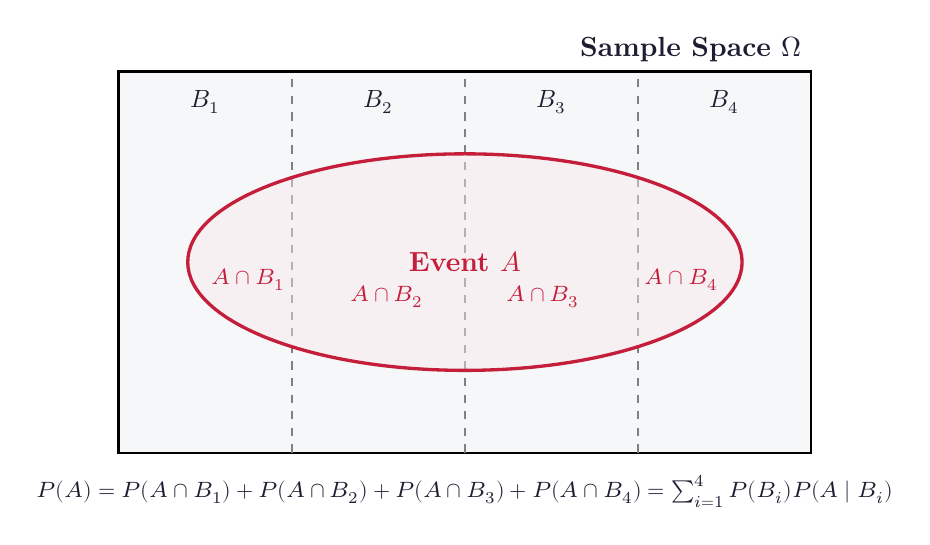
\begin{tikzpicture}[scale=1.1, every node/.style={font=\small}]
  % Sample space Omega rectangle
  \draw[thick, fill=mygray] (-4, -2.2) rectangle (4, 2.2);
  \node[above left, color=mydark, font=\bfseries] at (4, 2.2) {Sample Space $\Omega$};

  % Partition vertical dashed lines
  \draw[thick, dashed, color=gray] (-2, -2.2) -- (-2, 2.2);
  \draw[thick, dashed, color=gray] (0, -2.2) -- (0, 2.2);
  \draw[thick, dashed, color=gray] (2, -2.2) -- (2, 2.2);

  % Partition labels
  \node[above, color=mydark] at (-3, 1.6) {$B_1$};
  \node[above, color=mydark] at (-1, 1.6) {$B_2$};
  \node[above, color=mydark] at (1, 1.6) {$B_3$};
  \node[above, color=mydark] at (3, 1.6) {$B_4$};

  % Event A ellipse intersecting all partitions
  \draw[very thick, color=myred, fill=hdrred, fill opacity=0.45] (0, 0) ellipse (3.2cm and 1.25cm);
  \node[color=myred, font=\bfseries] at (0, 0) {Event $A$};

  % Slices of A in each partition
  \node[color=myred, font=\footnotesize] at (-2.5, -0.2) {$A \cap B_1$};
  \node[color=myred, font=\footnotesize] at (-0.9, -0.4) {$A \cap B_2$};
  \node[color=myred, font=\footnotesize] at (0.9, -0.4) {$A \cap B_3$};
  \node[color=myred, font=\footnotesize] at (2.5, -0.2) {$A \cap B_4$};

  % Caption
  \node[below, color=mydark, font=\footnotesize] at (0, -2.35) {
    $P(A) = P(A \cap B_1) + P(A \cap B_2) + P(A \cap B_3) + P(A \cap B_4) = \sum_{i=1}^4 P(B_i) P(A \mid B_i)$
  };
\end{tikzpicture}
\end{center}
\end{tcolorbox}

% ───────────────────────────────────────────────────────────────────────────────
\section{Discrete Random Variables, PMF and CDF}
% ───────────────────────────────────────────────────────────────────────────────

\begin{tcolorbox}[defbox, title={\textbf{Definition: Discrete Random Variable}}]
A \textbf{random variable (RV)} $X$ is a real-valued measurable function mapping the sample space into the real line:
\begin{equation}
  X: \Omega \longrightarrow \mathbb{R}
\end{equation}
A random variable is called \textbf{discrete} if its range $R_X = X(\Omega)$ is a finite or countably infinite set $\{x_1, x_2, x_3, \dots\}$.
\end{tcolorbox}

\subsection{Probability Mass Function (PMF)}
The \textbf{Probability Mass Function (PMF)} assigns probabilities directly to individual realization values $x_i$:
\begin{equation}
  p_X(x_i) = P(X = x_i) = P(\{\omega \in \Omega : X(\omega) = x_i\})
\end{equation}
Every valid discrete PMF must satisfy two fundamental conditions:
\begin{enumerate}[leftmargin=*, itemsep=2pt]
  \item \textbf{Non-negativity:} $p_X(x_i) \ge 0 \quad \forall x_i \in R_X$
  \item \textbf{Unit Normalization:} $\sum_{i} p_X(x_i) = 1$
\end{enumerate}

\subsection{Cumulative Distribution Function (CDF)}
The \textbf{Cumulative Distribution Function (CDF)}, denoted by $F_X(x)$, defines the probability that the random variable $X$ takes on a value less than or equal to a specified threshold $x \in \mathbb{R}$:
\begin{equation}
  F_X(x) = P(X \le x) = \sum_{x_i \le x} p_X(x_i)
\end{equation}

\begin{tcolorbox}[formulabox, title={\textbf{Mathematical Properties of the Discrete CDF}}]
The CDF $F_X(x)$ of any discrete random variable satisfies:
\begin{enumerate}[leftmargin=*, itemsep=3pt]
  \item \textbf{Boundary Limits:} $\displaystyle\lim_{x \to -\infty} F_X(x) = 0 \quad \text{and} \quad \lim_{x \to +\infty} F_X(x) = 1$
  \item \textbf{Monotonic Non-Decreasing:} If $a < b$, then $F_X(a) \le F_X(b)$.
  \item \textbf{Right-Continuity:} $\displaystyle\lim_{h \to 0^+} F_X(x + h) = F_X(x)$
  \item \textbf{Step Discontinuities (Jump Heights):} At every point $x_k$ with non-zero mass $p_X(x_k) > 0$, $F_X(x)$ exhibits a jump discontinuity of magnitude equal to the PMF:
  \begin{equation}
    P(X = x_k) = F_X(x_k) - F_X(x_k^-) = F_X(x_k) - \lim_{\epsilon \to 0^+} F_X(x_k - \epsilon)
  \end{equation}
  \item \textbf{Interval Probabilities:}
  \begin{align}
    P(a < X \le b) &= F_X(b) - F_X(a) \\[2pt]
    P(a \le X \le b) &= F_X(b) - F_X(a^-) = F_X(b) - F_X(a) + P(X = a)
  \end{align}
\end{enumerate}
\end{tcolorbox}

\begin{tcolorbox}[tikzbox, title={\textbf{TikZ Illustration: Discrete PMF Stems and Corresponding Staircase CDF}}]
\begin{center}
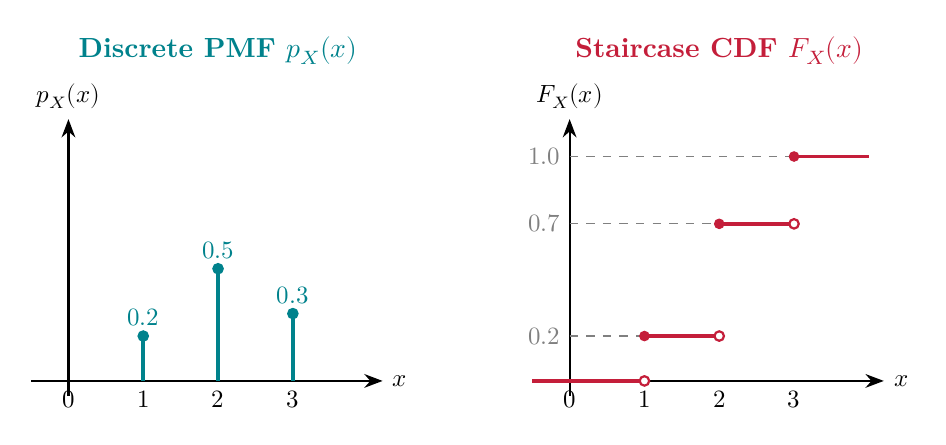
\begin{tikzpicture}[scale=0.95, every node/.style={font=\small}]
  % Left side: PMF
  \begin{scope}[shift={(-4.2,0)}]
    \draw[-Stealth, thick] (-0.5,0) -- (4.2,0) node[right] {$x$};
    \draw[-Stealth, thick] (0,-0.2) -- (0,3.5) node[above] {$p_X(x)$};

    % Stems
    \draw[line width=1.5pt, color=myteal] (1,0) -- (1,0.6);
    \filldraw[color=myteal] (1,0.6) circle (2pt) node[above] {$0.2$};
    \node[below] at (1,0) {$1$};

    \draw[line width=1.5pt, color=myteal] (2,0) -- (2,1.5);
    \filldraw[color=myteal] (2,1.5) circle (2pt) node[above] {$0.5$};
    \node[below] at (2,0) {$2$};

    \draw[line width=1.5pt, color=myteal] (3,0) -- (3,0.9);
    \filldraw[color=myteal] (3,0.9) circle (2pt) node[above] {$0.3$};
    \node[below] at (3,0) {$3$};

    \node[below] at (0,0) {$0$};
    \node[above, color=myteal, font=\bfseries] at (2.0, 4.1) {Discrete PMF $p_X(x)$};
  \end{scope}

  % Right side: CDF Staircase
  \begin{scope}[shift={(2.5,0)}]
    \draw[-Stealth, thick] (-0.5,0) -- (4.2,0) node[right] {$x$};
    \draw[-Stealth, thick] (0,-0.2) -- (0,3.5) node[above] {$F_X(x)$};

    % Levels: 0 before x=1, 0.2 from 1 to 2, 0.7 from 2 to 3, 1.0 for x >= 3
    % y-axis ticks: 0.2 -> 0.6, 0.7 -> 2.1, 1.0 -> 3.0
    \draw[dashed, color=gray] (0, 0.6) node[left] {$0.2$} -- (1, 0.6);
    \draw[dashed, color=gray] (0, 2.1) node[left] {$0.7$} -- (2, 2.1);
    \draw[dashed, color=gray] (0, 3.0) node[left] {$1.0$} -- (3, 3.0);

    % Stair segments
    \draw[very thick, color=myred] (-0.5, 0) -- (1, 0);
    \draw[fill=white, draw=myred, thick] (1,0) circle (1.8pt);

    \draw[very thick, color=myred] (1, 0.6) -- (2, 0.6);
    \filldraw[color=myred] (1, 0.6) circle (1.8pt);
    \draw[fill=white, draw=myred, thick] (2, 0.6) circle (1.8pt);

    \draw[very thick, color=myred] (2, 2.1) -- (3, 2.1);
    \filldraw[color=myred] (2, 2.1) circle (1.8pt);
    \draw[fill=white, draw=myred, thick] (3, 2.1) circle (1.8pt);

    \draw[very thick, color=myred] (3, 3.0) -- (4.0, 3.0);
    \filldraw[color=myred] (3, 3.0) circle (1.8pt);

    % Ticks on x-axis
    \node[below] at (1,0) {$1$};
    \node[below] at (2,0) {$2$};
    \node[below] at (3,0) {$3$};
    \node[below] at (0,0) {$0$};

    \node[above, color=myred, font=\bfseries] at (2.0, 4.1) {Staircase CDF $F_X(x)$};
  \end{scope}
\end{tikzpicture}
\end{center}
\end{tcolorbox}

% ───────────────────────────────────────────────────────────────────────────────
\section{Expectation, Moments, Variance, Covariance and Correlation}
% ───────────────────────────────────────────────────────────────────────────────

\begin{tcolorbox}[defbox, title={\textbf{Definition: Mathematical Expectation of a Discrete RV}}]
Let $X$ be a discrete random variable with PMF $p_X(x)$. The \textbf{expected value} (or mathematical expectation / first raw moment) of $X$ is defined as:
\begin{equation}
  E[X] = \mu = \sum_{x \in R_X} x \cdot p_X(x)
\end{equation}
provided that the series converges absolutely: $\sum_{x} |x| p_X(x) < \infty$. If the series diverges, the expectation does not exist.
\end{tcolorbox}

\subsection{Properties of Mathematical Expectation}
For arbitrary constants $a, b \in \mathbb{R}$ and measurable functions $g(X), h(X)$:
\begin{enumerate}[leftmargin=*, itemsep=3pt]
  \item \textbf{Expectation of a Constant:} $E[c] = c \sum p_X(x) = c$.
  \item \textbf{Linearity of Expectation:} For any random variables $X$ and $Y$ (independent or dependent!):
  \begin{equation}
    E[aX + bY + c] = aE[X] + bE[Y] + c
  \end{equation}
  \item \textbf{Law of the Unconscious Statistician (LOTUS):} For any function $g(X)$:
  \begin{equation}
    E[g(X)] = \sum_{x \in R_X} g(x) \cdot p_X(x)
  \end{equation}
  \item \textbf{Product Rule for Independent RVs:} If $X$ and $Y$ are independent:
  \begin{equation}
    E[X \cdot Y] = E[X] \cdot E[Y]
  \end{equation}
\end{enumerate}

\subsection{Moments: Raw Moments and Central Moments}
\begin{itemize}[leftmargin=*, itemsep=3pt]
  \item \textbf{$r$-th Raw Moment ($\mu_r'$):} Expectation about the origin:
  \begin{equation}
    \mu_r' = E[X^r] = \sum_{x} x^r p_X(x), \quad \mu_1' = \mu = E[X]
  \end{equation}
  \item \textbf{$r$-th Central Moment ($\mu_r$):} Expectation about the mean $\mu$:
  \begin{equation}
    \mu_r = E[(X - \mu)^r] = \sum_{x} (x - \mu)^r p_X(x)
  \end{equation}
  Specifically:
  \begin{align}
    \mu_0 &= E[(X-\mu)^0] = 1 \\[2pt]
    \mu_1 &= E[X - \mu] = E[X] - \mu = 0 \quad (\text{Always zero!}) \\[2pt]
    \mu_2 &= E[(X - \mu)^2] = \operatorname{Var}(X) = \sigma^2 \\[2pt]
    \mu_3 &= E[(X - \mu)^3] = \mu_3' - 3\mu_2'\mu + 2\mu^3 \quad (\text{Skewness measure}) \\[2pt]
    \mu_4 &= E[(X - \mu)^4] = \mu_4' - 4\mu_3'\mu + 6\mu_2'\mu^2 - 3\mu^4 \quad (\text{Kurtosis measure})
  \end{align}
\end{itemize}

\begin{tcolorbox}[formulabox, title={\textbf{Variance and Standard Deviation}}]
The \textbf{variance} of $X$, denoted $\operatorname{Var}(X)$ or $\sigma^2$, measures the degree of dispersion around the mean:
\begin{equation}
  \operatorname{Var}(X) = \sigma^2 = E\left[(X - E[X])^2\right] = E[X^2] - (E[X])^2 = \mu_2' - (\mu_1')^2
\end{equation}
\textbf{Fundamental Properties of Variance:}
\begin{enumerate}[leftmargin=*, itemsep=2pt]
  \item $\operatorname{Var}(X) \ge 0$, and $\operatorname{Var}(X) = 0 \iff X = c$ (constant with probability 1).
  \item $\operatorname{Var}(aX + b) = a^2 \operatorname{Var}(X)$. Adding a constant shifts position without altering spread!
  \item Standard deviation is $\sigma = \sqrt{\operatorname{Var}(X)}$, which retains the original units of $X$.
\end{enumerate}
\end{tcolorbox}

\begin{tcolorbox}[defbox, title={\textbf{Definition: Covariance and Correlation Coefficient}}]
\textbf{Covariance:} For two random variables $X$ and $Y$ with means $\mu_X$ and $\mu_Y$, their \textbf{covariance} is:
\begin{equation}
  \operatorname{Cov}(X, Y) = \sigma_{XY} = E[(X - \mu_X)(Y - \mu_Y)] = E[XY] - \mu_X \mu_Y
\end{equation}
\textbf{Pearson Correlation Coefficient ($\rho$):} Normalized measure of linear dependence:
\begin{equation}
  \rho(X, Y) = \frac{\operatorname{Cov}(X, Y)}{\sigma_X \sigma_Y} = \frac{E[XY] - E[X]E[Y]}{\sqrt{\operatorname{Var}(X)\operatorname{Var}(Y)}}
\end{equation}
\end{tcolorbox}

\subsection{Proof that \texorpdfstring{$-1 \le \rho \le 1$}{-1 <= rho <= 1}}
\begin{tcolorbox}[examplebox, title={\textbf{Rigorous Derivation: Cauchy-Schwarz Bound on Correlation}}]
Consider the standardized variables $U = \frac{X - \mu_X}{\sigma_X}$ and $V = \frac{Y - \mu_Y}{\sigma_Y}$. Clearly $E[U] = E[V] = 0$, $E[U^2] = E[V^2] = 1$, and $E[UV] = \rho$.
For any real scalar $t \in \mathbb{R}$, define the quadratic form:
\begin{equation}
  Q(t) = E\left[(t U + V)^2\right] \ge 0 \quad (\text{since the square of a real quantity is non-negative})
\end{equation}
Expanding the quadratic expectation:
\begin{align}
  Q(t) &= E\left[t^2 U^2 + 2t UV + V^2\right] \nonumber \\
       &= t^2 E[U^2] + 2t E[UV] + E[V^2] \nonumber \\
       &= t^2 (1) + 2t \rho + 1 \ge 0 \quad \forall t \in \mathbb{R}
\end{align}
For a quadratic $A t^2 + B t + C \ge 0$ with $A = 1 > 0$ to remain non-negative for all real $t$, its discriminant $\Delta = B^2 - 4AC$ must be non-positive:
\begin{equation}
  \Delta = (2\rho)^2 - 4(1)(1) \le 0 \implies 4\rho^2 - 4 \le 0 \implies \rho^2 \le 1
\end{equation}
Taking square roots yields:
\begin{equation}
  -1 \le \rho \le 1
\end{equation}
\begin{itemize}[leftmargin=*, itemsep=1pt]
  \item $\rho = +1$: Perfect positive linear relationship ($Y = aX + b$ with $a > 0$).
  \item $\rho = -1$: Perfect negative linear relationship ($Y = aX + b$ with $a < 0$).
  \item $\rho = 0$: $X$ and $Y$ are \textbf{uncorrelated}. Note: Independent $\implies$ Uncorrelated, but Uncorrelated does not imply Independent!
\end{itemize}
\end{tcolorbox}

\subsection{Variance of a Sum of Random Variables}
For $n$ random variables $X_1, X_2, \dots, X_n$:
\begin{equation}
  \operatorname{Var}\left(\sum_{i=1}^n X_i\right) = \sum_{i=1}^n \operatorname{Var}(X_i) + 2 \sum_{1 \le i < j \le n} \operatorname{Cov}(X_i, X_j)
\end{equation}
For two variables:
\begin{equation}
  \operatorname{Var}(aX \pm bY) = a^2 \operatorname{Var}(X) + b^2 \operatorname{Var}(Y) \pm 2ab \operatorname{Cov}(X, Y)
\end{equation}
If $X$ and $Y$ are independent (or merely uncorrelated so that $\operatorname{Cov}(X,Y) = 0$):
\begin{equation}
  \operatorname{Var}(X + Y) = \operatorname{Var}(X - Y) = \operatorname{Var}(X) + \operatorname{Var}(Y)
\end{equation}

% ───────────────────────────────────────────────────────────────────────────────
\section{Bernoulli Trials, Multinomial, Poisson Approximation \& Convolutions}
% ───────────────────────────────────────────────────────────────────────────────

\subsection{Bernoulli Trials and Binomial Distribution}
A \textbf{Bernoulli trial} is an experiment with exactly two mutually exclusive outcomes: \textit{Success} ($S$) with probability $p$, and \textit{Failure} ($F$) with probability $q = 1 - p$.
In a sequence of $n$ independent and identical Bernoulli trials:
\begin{tcolorbox}[formulabox, title={\textbf{Binomial Distribution $\mathbf{Bin(n, p)}$}}]
The random variable $X$, representing the total number of successes in $n$ trials, follows the Binomial distribution:
\begin{equation}
  P(X = k) = \binom{n}{k} p^k q^{n-k} = \frac{n!}{k!(n-k)!} p^k (1-p)^{n-k}, \quad k \in \{0, 1, 2, \dots, n\}
\end{equation}
Statistical parameters:
\begin{equation}
  E[X] = np, \qquad \operatorname{Var}(X) = npq = np(1-p), \qquad \sigma_X = \sqrt{np(1-p)}
\end{equation}
Since $q = 1-p < 1$, the variance of a Binomial distribution is strictly less than its mean: $\operatorname{Var}(X) < E[X]$.
\end{tcolorbox}

\subsection{Multinomial Distribution}
The \textbf{Multinomial distribution} generalizes the Binomial distribution to trials having $k \ge 2$ mutually exclusive outcomes $E_1, E_2, \dots, E_k$ with respective constant probabilities $p_1, p_2, \dots, p_k$ where $\sum_{j=1}^k p_j = 1$.
\begin{tcolorbox}[defbox, title={\textbf{Definition: Multinomial PMF}}]
In $n$ independent repetitions, let $X_j$ denote the number of times event $E_j$ occurs ($\sum_{j=1}^k X_j = n$). The joint PMF is:
\begin{equation}
  P(X_1 = x_1, X_2 = x_2, \dots, X_k = x_k) = \frac{n!}{x_1! x_2! \cdots x_k!} p_1^{x_1} p_2^{x_2} \cdots p_k^{x_k}
\end{equation}
where $x_j \in \{0, 1, \dots, n\}$ and $\sum_{j=1}^k x_j = n$.
\textbf{Moments and Covariances:}
\begin{equation}
  E[X_j] = n p_j, \qquad \operatorname{Var}(X_j) = n p_j (1 - p_j), \qquad \operatorname{Cov}(X_i, X_j) = -n p_i p_j \quad (i \ne j)
\end{equation}
\textit{Key Insight:} Covariance is strictly negative because an increase in occurrences of event $E_i$ constrains the remaining trials available for event $E_j$.
\end{tcolorbox}

\subsection{Poisson Approximation to the Binomial Distribution (Law of Rare Events)}
When the number of trials $n$ is very large ($n \to \infty$) and the success probability $p$ is very small ($p \to 0$) such that the average occurrence rate $\lambda = np$ remains a finite positive constant:
\begin{tcolorbox}[examplebox, title={\textbf{Rigorous Derivation: Poisson Limit Theorem}}]
Starting from the Binomial PMF:
\begin{equation}
  P(X = k) = \binom{n}{k} p^k (1-p)^{n-k} = \frac{n(n-1)(n-2)\cdots(n-k+1)}{k!} \left(\frac{\lambda}{n}\right)^k \left(1 - \frac{\lambda}{n}\right)^{n-k}
\end{equation}
Rearranging terms:
\begin{equation}
  P(X = k) = \frac{\lambda^k}{k!} \cdot \left[\frac{n}{n} \cdot \frac{n-1}{n} \cdot \frac{n-2}{n} \cdots \frac{n-k+1}{n}\right] \cdot \left(1 - \frac{\lambda}{n}\right)^n \cdot \left(1 - \frac{\lambda}{n}\right)^{-k}
\end{equation}
Taking the limit as $n \to \infty$ for fixed $k$:
\begin{align}
  \lim_{n \to \infty} \left(1 - \frac{1}{n}\right)\left(1 - \frac{2}{n}\right)\cdots\left(1 - \frac{k-1}{n}\right) &= 1 \cdot 1 \cdots 1 = 1 \\[3pt]
  \lim_{n \to \infty} \left(1 - \frac{\lambda}{n}\right)^n &= e^{-\lambda} \\[3pt]
  \lim_{n \to \infty} \left(1 - \frac{\lambda}{n}\right)^{-k} &= (1 - 0)^{-k} = 1
\end{align}
Multiplying these limits:
\begin{equation}
  \lim_{n \to \infty} P(X = k) = \frac{\lambda^k e^{-\lambda}}{k!}, \qquad k = 0, 1, 2, \dots
\end{equation}
This is the PMF of the \textbf{Poisson distribution} with parameter $\lambda = np$. For Poisson, $E[X] = \operatorname{Var}(X) = \lambda$.
\end{tcolorbox}

\begin{tcolorbox}[tikzbox, title={\textbf{TikZ Plot: Binomial PMF ($n=20, p=0.1$) vs. Poisson PMF ($\lambda = np = 2.0$)}}]
\begin{center}
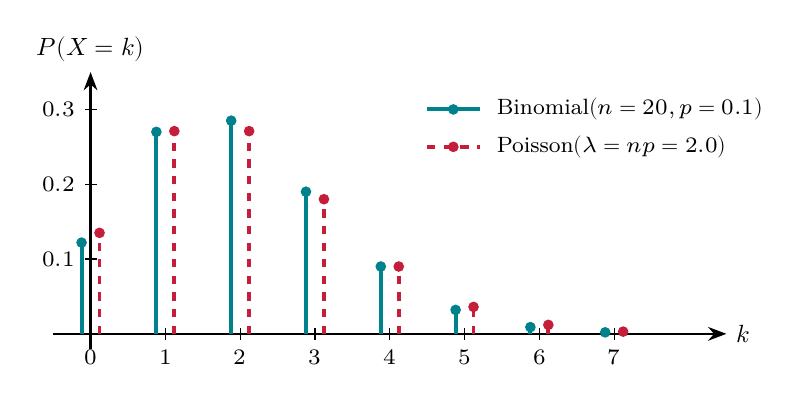
\begin{tikzpicture}[scale=0.95, every node/.style={font=\small}]
  % Axes
  \draw[-Stealth, thick] (-0.5, 0) -- (8.5, 0) node[right] {$k$};
  \draw[-Stealth, thick] (0, -0.2) -- (0, 3.5) node[above] {$P(X=k)$};

  % Ticks on x-axis
  \foreach \x in {0,1,2,3,4,5,6,7} {
    \draw (\x, 0.08) -- (\x, -0.08) node[below] {\footnotesize $\x$};
  }

  % Ticks on y-axis (scale: prob 0.3 -> y=3.0)
  \draw (0.08, 1.0) -- (-0.08, 1.0) node[left] {\footnotesize $0.1$};
  \draw (0.08, 2.0) -- (-0.08, 2.0) node[left] {\footnotesize $0.2$};
  \draw (0.08, 3.0) -- (-0.08, 3.0) node[left] {\footnotesize $0.3$};

  % Data: (k, Binomial P, Poisson P)
  % k=0: Bin=0.1216 (1.22), Poi=0.1353 (1.35)
  % k=1: Bin=0.2702 (2.70), Poi=0.2707 (2.71)
  % k=2: Bin=0.2852 (2.85), Poi=0.2707 (2.71)
  % k=3: Bin=0.1901 (1.90), Poi=0.1804 (1.80)
  % k=4: Bin=0.0898 (0.90), Poi=0.0902 (0.90)
  % k=5: Bin=0.0319 (0.32), Poi=0.0361 (0.36)
  % k=6: Bin=0.0089 (0.09), Poi=0.0120 (0.12)
  % k=7: Bin=0.0020 (0.02), Poi=0.0034 (0.03)

  % Binomial stems (blue/teal, offset -0.1)
  \foreach \k/\h in {0/1.22, 1/2.70, 2/2.85, 3/1.90, 4/0.90, 5/0.32, 6/0.09, 7/0.02} {
    \draw[line width=1.4pt, color=myteal] ({\k-0.12}, 0) -- ({\k-0.12}, \h);
    \filldraw[color=myteal] ({\k-0.12}, \h) circle (1.8pt);
  }

  % Poisson stems (red/dashed, offset +0.1)
  \foreach \k/\h in {0/1.35, 1/2.71, 2/2.71, 3/1.80, 4/0.90, 5/0.36, 6/0.12, 7/0.03} {
    \draw[line width=1.4pt, color=myred, dashed] ({\k+0.12}, 0) -- ({\k+0.12}, \h);
    \filldraw[color=myred] ({\k+0.12}, \h) circle (1.8pt);
  }

  % Legend
  \draw[line width=1.4pt, color=myteal] (4.5, 3.0) -- (5.2, 3.0);
  \filldraw[color=myteal] (4.85, 3.0) circle (1.8pt);
  \node[right, font=\footnotesize] at (5.3, 3.0) {$\text{Binomial}(n=20, p=0.1)$};

  \draw[line width=1.4pt, color=myred, dashed] (4.5, 2.5) -- (5.2, 2.5);
  \filldraw[color=myred] (4.85, 2.5) circle (1.8pt);
  \node[right, font=\footnotesize] at (5.3, 2.5) {$\text{Poisson}(\lambda = np = 2.0)$};
\end{tikzpicture}
\end{center}
\end{tcolorbox}

\subsection{Infinite Sequences of Bernoulli Trials: Geometric Distribution}
When independent Bernoulli trials are repeated indefinitely until the \textbf{first success} occurs:
\begin{equation}
  P(X = k) = (1-p)^{k-1} p = q^{k-1} p, \qquad k \in \{1, 2, 3, \dots\}
\end{equation}
Properties of the \textbf{Geometric distribution}:
\begin{equation}
  E[X] = \frac{1}{p}, \qquad \operatorname{Var}(X) = \frac{1-p}{p^2} = \frac{q}{p^2}
\end{equation}
\textbf{Memoryless Property:} The geometric distribution is the \textit{only} discrete distribution possessing memorylessness:
\begin{equation}
  P(X > s + t \mid X > s) = P(X > t) \quad \forall s, t \in \mathbb{N}
\end{equation}

\subsection{Sums of Independent Random Variables (Discrete Convolution)}
Let $X$ and $Y$ be independent discrete integer-valued random variables with PMFs $p_X(x)$ and $p_Y(y)$. The PMF of their sum $Z = X + Y$ is obtained via \textbf{discrete convolution}:
\begin{equation}
  p_Z(z) = P(Z = z) = \sum_{k=-\infty}^\infty P(X = k, Y = z - k) = \sum_{k=-\infty}^\infty p_X(k) \cdot p_Y(z - k) = (p_X * p_Y)(z)
\end{equation}
\begin{tcolorbox}[formulabox, title={\textbf{Reproductive (Convolution) Properties of Key Discrete Distributions}}]
\begin{enumerate}[leftmargin=*, itemsep=3pt]
  \item \textbf{Sum of Independent Binomials:} If $X \sim \text{Bin}(n_1, p)$ and $Y \sim \text{Bin}(n_2, p)$ share the same success parameter $p$:
  \begin{equation}
    Z = X + Y \sim \text{Bin}(n_1 + n_2, p)
  \end{equation}
  \item \textbf{Sum of Independent Poissons:} If $X \sim \text{Poisson}(\lambda_1)$ and $Y \sim \text{Poisson}(\lambda_2)$:
  \begin{equation}
    Z = X + Y \sim \text{Poisson}(\lambda_1 + \lambda_2)
  \end{equation}
  \textit{Proof Sketch:} Using the convolution formula:
  \begin{equation}
    P(Z = z) = \sum_{k=0}^z \frac{e^{-\lambda_1} \lambda_1^k}{k!} \cdot \frac{e^{-\lambda_2} \lambda_2^{z-k}}{(z-k)!} = \frac{e^{-(\lambda_1+\lambda_2)}}{z!} \sum_{k=0}^z \binom{z}{k} \lambda_1^k \lambda_2^{z-k} = \frac{e^{-(\lambda_1+\lambda_2)} (\lambda_1+\lambda_2)^z}{z!}
  \end{equation}
\end{enumerate}
\end{tcolorbox}

% ───────────────────────────────────────────────────────────────────────────────
\section{Chebyshev's Inequality and Concentration Bounds}
% ───────────────────────────────────────────────────────────────────────────────

When the exact probability distribution of a random variable is unknown, Chebyshev's Inequality provides a guaranteed mathematical upper bound on the probability of significant deviations from the mean, requiring knowledge of only the mean $\mu$ and finite variance $\sigma^2$.

\begin{tcolorbox}[defbox, title={\textbf{Markov's Inequality (Foundation for Chebyshev)}}]
If $Y$ is a non-negative random variable ($P(Y \ge 0) = 1$) with finite expectation $E[Y] < \infty$, then for any positive real constant $a > 0$:
\begin{equation}
  P(Y \ge a) \le \frac{E[Y]}{a}
\end{equation}
\textbf{Proof:}
\begin{equation}
  E[Y] = \sum_{y} y p_Y(y) = \sum_{y < a} y p_Y(y) + \sum_{y \ge a} y p_Y(y) \ge \sum_{y \ge a} y p_Y(y) \ge a \sum_{y \ge a} p_Y(y) = a P(Y \ge a)
\end{equation}
Dividing both sides by $a > 0$ completes the proof.
\end{tcolorbox}

\begin{tcolorbox}[examplebox, title={\textbf{Rigorous Derivation of Chebyshev's Inequality}}]
Let $X$ be any random variable with mean $\mu = E[X]$ and variance $\sigma^2 = \operatorname{Var}(X) < \infty$.
Define the non-negative random variable $Y = (X - \mu)^2 \ge 0$.
Applying Markov's inequality to $Y$ with threshold $a = \epsilon^2$ (where $\epsilon > 0$):
\begin{equation}
  P\left(Y \ge \epsilon^2\right) \le \frac{E[Y]}{\epsilon^2} \implies P\left((X - \mu)^2 \ge \epsilon^2\right) \le \frac{E\left[(X - \mu)^2\right]}{\epsilon^2}
\end{equation}
Since $(X - \mu)^2 \ge \epsilon^2 \iff |X - \mu| \ge \epsilon$, and $E[(X - \mu)^2] = \sigma^2$:
\begin{equation}
  P(|X - \mu| \ge \epsilon) \le \frac{\sigma^2}{\epsilon^2}
\end{equation}
Substituting $\epsilon = k\sigma$ (where $k > 0$ represents the deviation in units of standard deviations):
\begin{equation}
  P(|X - \mu| \ge k\sigma) \le \frac{1}{k^2}
\end{equation}
Taking the complementary event yields the dual form:
\begin{equation}
  P(|X - \mu| < k\sigma) \ge 1 - \frac{1}{k^2}
\end{equation}
\end{tcolorbox}

\begin{tcolorbox}[tikzbox, title={\textbf{TikZ Schematic: Geometric Interpretation of Chebyshev's Concentration Bound}}]
\begin{center}
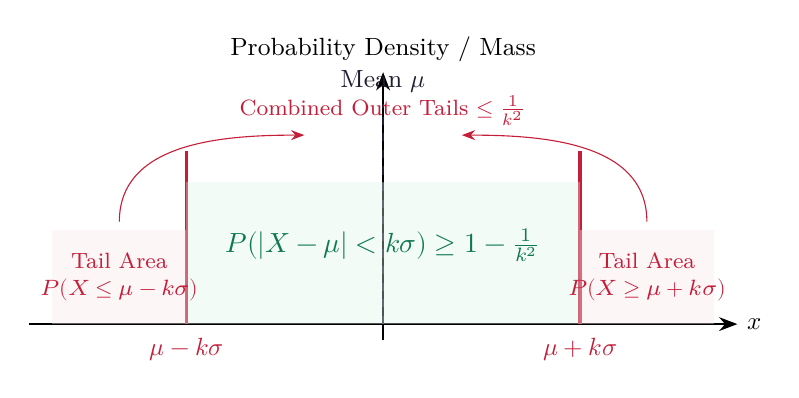
\begin{tikzpicture}[scale=1.0, every node/.style={font=\small}]
  % Axis
  \draw[-Stealth, thick] (-4.5, 0) -- (4.5, 0) node[right] {$x$};
  \draw[-Stealth, thick] (0, -0.2) -- (0, 3.2) node[above] {Probability Density / Mass};

  % Mean center line
  \draw[thick, dashed, color=mydark] (0, 0) -- (0, 2.8) node[above] {Mean $\mu$};

  % Symmetric bounds: mu - k*sigma and mu + k*sigma
  \draw[very thick, color=myred] (-2.5, 0) -- (-2.5, 2.2);
  \node[below, color=myred] at (-2.5, -0.05) {$\mu - k\sigma$};

  \draw[very thick, color=myred] (2.5, 0) -- (2.5, 2.2);
  \node[below, color=myred] at (2.5, -0.05) {$\mu + k\sigma$};

  % Shaded central interval
  \fill[fill=hdrgreen, fill opacity=0.35] (-2.5, 0) rectangle (2.5, 1.8);
  \node[color=mygreen, font=\bfseries] at (0, 1.0) {$P(|X - \mu| < k\sigma) \ge 1 - \frac{1}{k^2}$};

  % Shaded outer tails
  \fill[fill=hdrred, fill opacity=0.4] (-4.2, 0) rectangle (-2.5, 1.2);
  \fill[fill=hdrred, fill opacity=0.4] (2.5, 0) rectangle (4.2, 1.2);
  \node[color=myred, font=\footnotesize, align=center] at (-3.35, 0.6) {Tail Area\\$P(X \le \mu - k\sigma)$};
  \node[color=myred, font=\footnotesize, align=center] at (3.35, 0.6) {Tail Area\\$P(X \ge \mu + k\sigma)$};

  % Total tail bound note
  \draw[-Stealth, thin, color=myred] (-3.35, 1.3) to[out=90, in=180] (-1.0, 2.4);
  \draw[-Stealth, thin, color=myred] (3.35, 1.3) to[out=90, in=0] (1.0, 2.4);
  \node[above, color=myred, font=\footnotesize] at (0, 2.4) {Combined Outer Tails $\le \frac{1}{k^2}$};
\end{tikzpicture}
\end{center}
\end{tcolorbox}

\subsection{Numerical Significance of Chebyshev's Bound}
\par\vspace{6pt}\noindent
\begingroup
\setlength{\tabcolsep}{6pt}
\setlength{\extrarowheight}{3pt}
\begin{tabularx}{\linewidth}{|B{2.2cm}|B{3.8cm}|B{4.0cm}|Y|}
\hline
\textbf{Spread ($k$)} & \textbf{Interval $[\mu - k\sigma, \mu + k\sigma]$} & \textbf{Chebyshev Bound ($P \ge 1 - 1/k^2$)} & \textbf{Normal Distribution Comparison} \\
\hline
$k = 1$ & $[\mu - \sigma, \mu + \sigma]$ & $\ge 0\%$ (Trivial bound) & $\approx 68.27\%$ \\
\hline
$k = 2$ & $[\mu - 2\sigma, \mu + 2\sigma]$ & $\ge 1 - 1/4 = 75.00\%$ & $\approx 95.45\%$ \\
\hline
$k = 3$ & $[\mu - 3\sigma, \mu + 3\sigma]$ & $\ge 1 - 1/9 = 88.89\%$ & $\approx 99.73\%$ \\
\hline
$k = 4$ & $[\mu - 4\sigma, \mu + 4\sigma]$ & $\ge 1 - 1/16 = 93.75\%$ & $\approx 99.9937\%$ \\
\hline
\end{tabularx}
\endgroup
\vspace{12pt}

\newpage
% ===============================================================================
% MANDATORY QUICK REVISION PAGE
% ===============================================================================
\begin{center}
  {\large\bfseries\color{myred} Quick Revision --- Module 1}\\[2pt]
  {\small\color{mydark} Basic Probability, Discrete Random Variables and Inequalities $|$ BS-M301}
\end{center}
\noindent{\color{myred}\rule{\linewidth}{1.0pt}}
\vspace{2pt}

\begin{tcolorbox}[formulabox, top=3pt, bottom=3pt, title={\textbf{Key Formulas and Probability Identities at a Glance}}]
\renewcommand{\arraystretch}{1.10}
\begin{tabularx}{\linewidth}{B{4.8cm} X}
Kolmogorov Axioms & $P(A) \ge 0, \quad P(\Omega) = 1, \quad P\left(\bigcup_{i=1}^\infty A_i\right) = \sum_{i=1}^\infty P(A_i) \text{ (disjoint)}$ \\[1pt]
Addition Law & $P(A \cup B) = P(A) + P(B) - P(A \cap B)$ \\[1pt]
Conditional Probability & $P(A \mid B) = \frac{P(A \cap B)}{P(B)}, \quad P(A \cap B) = P(A) \cdot P(B) \text{ (Independence)}$ \\[1pt]
Total Probability & $P(A) = \sum_{i=1}^n P(B_i) P(A \mid B_i) \quad (\text{Partition } \{B_i\})$ \\[1pt]
Bayes' Theorem & $P(B_k \mid A) = \frac{P(B_k) P(A \mid B_k)}{\sum_{i=1}^n P(B_i) P(A \mid B_i)}$ \\[1pt]
Discrete Expectation & $E[X] = \mu = \sum_x x p_X(x), \quad E[aX + bY] = aE[X] + bE[Y]$ \\[1pt]
Variance Formula & $\operatorname{Var}(X) = \sigma^2 = E[X^2] - (E[X])^2, \quad \operatorname{Var}(aX+b) = a^2 \operatorname{Var}(X)$ \\[1pt]
Covariance \& Correlation & $\operatorname{Cov}(X,Y) = E[XY] - \mu_X \mu_Y, \quad \rho = \frac{\operatorname{Cov}(X,Y)}{\sigma_X \sigma_Y} \in [-1, 1]$ \\[1pt]
Binomial Distribution & $P(X=k) = \binom{n}{k} p^k q^{n-k}, \quad \mu = np, \; \sigma^2 = npq$ \\[1pt]
Poisson Approximation & $P(X=k) = \frac{\lambda^k e^{-\lambda}}{k!}, \quad \lambda = np, \; \mu = \sigma^2 = \lambda$ \\[1pt]
Chebyshev's Inequality & $P(|X - \mu| \ge k\sigma) \le \frac{1}{k^2}, \quad P(|X - \mu| < k\sigma) \ge 1 - \frac{1}{k^2}$ \\
\end{tabularx}
\end{tcolorbox}

\vspace{1pt}

\begin{tcolorbox}[defbox, top=3pt, bottom=3pt, title={\textbf{One-Line Definitions}}]
\begin{itemize}[leftmargin=*, itemsep=0.5pt, topsep=0pt]
  \item \textbf{Probability Space $(\Omega, \mathcal{F}, P)$:} Formal triplet of sample space, $\sigma$-algebra of events, and Kolmogorov measure.
  \item \textbf{$\sigma$-algebra ($\mathcal{F}$):} Event collection closed under complementation and countable unions containing $\Omega$.
  \item \textbf{Statistical Independence:} Condition where $P(A \cap B) = P(A)P(B)$, giving zero mutual information.
  \item \textbf{Random Variable:} A measurable real-valued function $X: \Omega \to \mathbb{R}$ mapping outcomes to real numbers.
  \item \textbf{Probability Mass Function (PMF):} Discrete assignment $p_X(x) = P(X=x)$ with non-negativity and unit sum.
  \item \textbf{Cumulative Distribution Function (CDF):} Non-decreasing right-continuous probability $F_X(x) = P(X \le x)$.
  \item \textbf{Law of Rare Events:} Poisson convergence of Binomial distribution when $n \to \infty, p \to 0$ with $\lambda = np$ constant.
  \item \textbf{Memoryless Property:} Invariance condition $P(X > s+t \mid X > s) = P(X > t)$, uniquely held by Geometric distribution.
  \item \textbf{Uncorrelated Variables:} Variables with zero covariance ($\operatorname{Cov}(X,Y) = 0, \rho = 0$), weaker than full independence.
  \item \textbf{Chebyshev's Bound:} Non-parametric inequality guaranteeing at least $(1 - 1/k^2)$ probability mass within $\mu \pm k\sigma$.
\end{itemize}
\end{tcolorbox}

\newpage

\begin{tcolorbox}[exambox, title={\textbf{Frequently Asked / Viva Questions (Part 1)}}]
\begin{enumerate}[topsep=0pt, label=\textbf{Q\arabic*.}, itemsep=3.2pt]
  \item \Q{State Kolmogorov's Axioms of Probability and derive $P(\emptyset) = 0$.}
  Axiom 1: $P(A) \ge 0$. Axiom 2: $P(\Omega) = 1$. Axiom 3: Countable additivity for pairwise disjoint events. Since $\Omega = \Omega \cup \emptyset$ with $\Omega \cap \emptyset = \emptyset$, Axiom 3 yields $P(\Omega) = P(\Omega) + P(\emptyset) \implies P(\emptyset) = 0$.

  \item \Q{Distinguish between pairwise independence and mutual independence with an example.}
  Pairwise independence requires $P(A_i \cap A_j) = P(A_i)P(A_j)$ for all pairs. Mutual independence additionally requires the product rule across all $k$-tuples up to all $n$ events. In Bernstein's example (tossing two coins, $A$: heads on coin 1, $B$: heads on coin 2, $C$: both same), events are pairwise independent but not mutually independent.

  \item \Q{State and prove the Law of Total Probability.}
  If $\{B_1, \dots, B_n\}$ partitions $\Omega$, then $A = A \cap \Omega = \bigcup_{i=1}^n (A \cap B_i)$. Because the partitions are disjoint, the slices $(A \cap B_i)$ are mutually exclusive. By additivity, $P(A) = \sum_{i=1}^n P(A \cap B_i) = \sum_{i=1}^n P(B_i) P(A \mid B_i)$.

  \item \Q{Under what physical conditions does the Binomial distribution tend to the Poisson distribution?}
  When the number of independent trials $n \to \infty$, the probability of success on each trial $p \to 0$, such that the expected average number of occurrences $\lambda = np$ remains a finite positive constant (the law of rare events).

  \item \Q{Prove that for any random variable with finite variance, $\operatorname{Var}(aX + b) = a^2 \operatorname{Var}(X)$.}
  $E[aX + b] = a\mu + b$. Then $\operatorname{Var}(aX + b) = E[((aX + b) - (a\mu + b))^2] = E[(a(X - \mu))^2] = E[a^2 (X - \mu)^2] = a^2 E[(X - \mu)^2] = a^2 \operatorname{Var}(X)$. Adding a constant shifts the distribution without affecting spread.

  \item \Q{Why is covariance negative for components of a Multinomial distribution?}
  In a multinomial distribution, $\sum_{j=1}^k X_j = n$ is fixed. If event $i$ occurs more frequently ($X_i > E[X_i]$), fewer trials remain available for other events ($X_j < E[X_j]$), creating a deterministic negative association: $\operatorname{Cov}(X_i, X_j) = -n p_i p_j < 0$.

  \item \Q{Does zero correlation ($\rho = 0$) imply independence of two random variables?}
  No! Independence implies uncorrelatedness ($\operatorname{Cov}(X, Y) = 0 \implies \rho = 0$), but the converse is not true in general. For example, if $X \sim U[-1, 1]$ and $Y = X^2$, then $E[X] = 0$ and $E[XY] = E[X^3] = 0$, giving $\operatorname{Cov}(X, Y) = 0$ and $\rho = 0$, yet $Y$ is completely deterministically dependent on $X$!
\end{enumerate}
\end{tcolorbox}

\newpage

\begin{tcolorbox}[exambox, top=3pt, bottom=3pt, title={\textbf{Frequently Asked / Viva Questions (Part 2)}}]
\begin{enumerate}[topsep=0pt, label=\textbf{Q\arabic*.}, itemsep=1.8pt, start=8]
  \item \Q{State and prove Chebyshev's Inequality using Markov's Inequality.}
  Markov's inequality for non-negative $Y \ge 0$ states $P(Y \ge a) \le E[Y]/a$. Defining $Y = (X - \mu)^2 \ge 0$ and setting $a = k^2 \sigma^2$: $P((X - \mu)^2 \ge k^2 \sigma^2) \le E[(X - \mu)^2] / (k^2 \sigma^2) = \sigma^2 / (k^2 \sigma^2) = 1/k^2$. Since $(X - \mu)^2 \ge k^2 \sigma^2 \iff |X - \mu| \ge k\sigma$, we obtain $P(|X - \mu| \ge k\sigma) \le 1/k^2$.

  \item \Q{What is the reproductive property of independent Poisson random variables?}
  The sum of two independent Poisson variables $X \sim \text{Poisson}(\lambda_1)$ and $Y \sim \text{Poisson}(\lambda_2)$ is itself a Poisson random variable with parameter $\lambda_1 + \lambda_2$. This follows from the binomial expansion within the discrete convolution sum.

  \item \Q{Explain the memoryless property of the Geometric distribution.}
  $P(X > s + t \mid X > s) = P(X > t)$ for integers $s, t \ge 1$. If $s$ consecutive failures have already occurred, the probability of requiring at least $t$ additional trials until the first success is identical to the initial probability of requiring at least $t$ trials. The system has no memory of past failures.
\end{enumerate}
\end{tcolorbox}

\vspace{2pt}

\begin{tcolorbox}[tikzbox, top=3pt, bottom=3pt, title={\textbf{Summary Matrix: Comprehensive Comparison of Discrete Probability Distributions}}]
\par\vspace{1pt}\noindent
\begingroup
\setlength{\tabcolsep}{3.5pt}
\setlength{\extrarowheight}{1.0pt}
\renewcommand{\arraystretch}{1.12}
\begin{tabularx}{\linewidth}{|B{2.5cm}|B{3.8cm}|B{2.2cm}|B{2.2cm}|Y|}
\hline
\textbf{Distribution} & \textbf{Probability Mass Function (PMF)} & \textbf{Mean ($E[X]$)} & \textbf{Variance ($\sigma^2$)} & \textbf{Special Characteristic} \\
\hline
Bernoulli & $P(X=x) = p^x (1-p)^{1-x}, \; x \in \{0, 1\}$ & $p$ & $p(1-p)$ & Single trial; basic building block. \\
\hline
Binomial & $P(X=k) = \binom{n}{k} p^k (1-p)^{n-k}$ & $np$ & $np(1-p)$ & $\sigma^2 < \mu$; independent repeated trials. \\
\hline
Poisson & $P(X=k) = \frac{\lambda^k e^{-\lambda}}{k!}, \; k \in \mathbb{N}_0$ & $\lambda$ & $\lambda$ & $\sigma^2 = \mu$; law of rare events. \\
\hline
Geometric & $P(X=k) = (1-p)^{k-1} p, \; k \in \mathbb{N}$ & $\frac{1}{p}$ & $\frac{1-p}{p^2}$ & Only memoryless discrete distribution. \\
\hline
Multinomial & $P(X_1=x_1,\dots) = \frac{n!}{\prod x_j!} \prod p_j^{x_j}$ & $n p_j$ & $n p_j (1 - p_j)$ & Negative covariance $\operatorname{Cov} = -n p_i p_j$. \\
\hline
\end{tabularx}
\endgroup
\end{tcolorbox}

\end{document}
